\documentclass[]{article}
\usepackage{hyperref}
\usepackage{cleveref}
\usepackage{graphicx}
\usepackage{svg}
\usepackage{url}
\usepackage{minted}
\usepackage{fullpage}

% Title Page
\title{Local Computing Cluster Resources}
\author{Qimin Yan Group}


\begin{document}
\maketitle

\begin{abstract}
	This article gives an overview of the computational resources of our research group. Currently, it consists of several independent compute nodes, as well as one SLURM computational cluster. Basic usage is discussed along with the neccessary steps to set up new nodes and construct new clusters.
\end{abstract}

\tableofcontents

\section{Available Computational Clusters}

Currently, we have one operational cluster, which will be referred to as QYG-C1 (or simply `the cluster') hereafter. QYG-C1 consists of the basic tree network shown schematically in \cref{qyg-c1-schematic} with current IP addresses. The head node connects to both the internet (through ethernet port enp36s0f1) and the local cluster (port enp36s0f0).

The global IP address of the head node (enp36s0f1) is determined dynamically via DHCP by our network administrators and the local IP address (enp36s0f0) is set statically by us. All other IP addresses in the LAN are set statically. The local connection of the head node connects to the switch which acts as a central hub for all of the other network resources, namely the Network Attached Storage (NAS), and the compute nodes. 


\begin{figure}[h!]
	\centering
	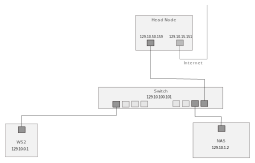
\includegraphics[scale=0.35]{qyg-c1-schem.pdf}
	\caption{A schematic detailing the basic tree architecture of QYG-C1.}\label{qyg-c1-schematic}
\end{figure}


The switch is a QNAP QSW-IM1200-8C and may be accessed and configured by connecting locally via an ethernet port and using the associated QNAP QFinder-Pro software. One may also access the switch by navigating to it's IP address in an internet browser on any locally connected device with an IP in it's subnet.

The NAS is an ASUSTOR which may be accessed and configured by connecting locally via an ethernet port and using the associated ASUSTOR Control Center software. One may also access the NAS by navigating to it's IP address in an internet browser on any locally connected device on it's subnet. The NAS incorporates a redundant memory scheme to safely store data and is currently configured to the RAID 5 standard. Note that the NAS's OS is not Ubuntu but instead ASUSTOR Data Master (ADM), a proprietary OS. Many basic linux commands and packages are included and useable in it's terminal environment, however.

Compute nodes consist of PCs each with a single Intel i9 CPU and four Nvidia RTX 4090 GPUs. Each has Ubuntu installed as the OS.




\section{Constructing a New Cluster}
The construction of a new SLURM computational cluster consists of three basic steps: \textit{(1)} constructing a Local Access Network (LAN); \textit{(2)} homogenizing users and software across nodes; and, \textit{(3)} installing SLURM and initializing it's daemons. Each of these basic steps are detailed in the following sections.

\subsection{Local Access Networks}
A local access network (LAN) is a set of devices that are locally connected (often physically via ethernet cables) such that each may communicate without access to the internet. For a computational cluster, physical connections (cables) are almost always preferred to reduce network latency (time for communication between devices).

Constructing a LAN is relatively easy: first all devices must be locally connected (of course), and then each must be assigned an IP address on the same subnet. The IP address range for a subnet may be determined by some given IP address (often a global IP address which allows for internet connection and is determined by some ISP or IT staff) and a subnet mask.

The first division of digits of an IP determine it's class. The class of an IP address determines it's subnet mask, and corresponding number of devices it may have on it's subnet. We are often given some IP address from an ISP or network administrator which we may then build a subnet on.

\subsubsection{Configuring Gateway}
In the basic tree architecture used here, only the head node has direct connection to the internet. Thus, other devices in the LAN need to use the head node as a gateway to access the internet. This may be configured with iptables and route commands. 
On the local node:
\begin{verbatim}
	sudo route add default gw 129.10.50.159
\end{verbatim}
On the gateway:
\begin{verbatim}
	 echo 1 > /proc/sys/net/ipv4/ip_forward
	 sudo iptables -t nat -A POSTROUTING -o enp36s0f1 -j MASQUERADE
	 sudo iptables -A FORWARD -i enp36s0f0 -o enp36s0f1 -j ACCEPT
	 sudo iptables -A FORWARD -i enp36s0f1 -o enp36s0f0  -m state --state RELATED,ESTABLISHED -j ACCEPT
\end{verbatim}
See \url{https://unix.stackexchange.com/questions/222054/how-can-i-use-linux-as-a-gateway}.
Current networking routes may be checked with the \verb|routel| command.

\subsubsection{Setting DNS Server on Subnodes}
A Domain Name System (DNS) is essentially a directory relating web addresses to IP addresses. For example, a DNS provides the map from the web address `www.google.com' to the IP address `8.8.8.8'. The head node has an IP address provided by our network administrator via a DHCP protocol that also provides a DNS server. 

Sub-nodes on the tree architecture used here may need to have their DNS servers updated or set manually, however. To set manually, see the file located at \verb|/etc/resolv.conf| and edit the IP address listed after \verb|nameserver|.
For more detail, see \url{https://www.geeksforgeeks.org/how-to-configure-dns-in-linux/}.

\subsubsection{Installing Packages on Nodes Without Direct Internet Access}

In the basic tree architecture of QYG-C1, only the head node has direct internet access. This allows for the head node to act as a global firewall for the network but does hinder some functions of the compute nodes. The following introduces a set of commands that allows for packages to be installed using apt on offline devices through online repositories accessible by the head node.

From the device with internet access, first SSH into the local device without internet access with:

\begin{verbatim}
	sudo ssh -R <selected port>:us.archive.ubuntu.com:80 user@nointernethost
\end{verbatim}
We then need to create a file (if it doesn't already exist) '/etc/apt/apt.conf' and add the following two lines:
\begin{verbatim}
	Acquire::http::Proxy "http://localhost:<selected port>";
	Acquire::https::Proxy "https://localhost:<selected port>";
\end{verbatim}
Running apt on the remote node without internet access should then allow us to download packages as long as the former ssh command is active. In consequent uses, the configuration file should be maintained, so that only the first ssh command is needed.
This chain of commands is based on: \url{https://stackoverflow.com/questions/36353955/apt-get-install- via-tunnel-proxy-but-ssh-only-from-client-side}. 

\subsection{Prerequisites for SLURM Installation}

A SLURM cluster requires a homogeneous set of users and specific software across all nodes in the cluster. Specifically, the user names and user ids (UIDs) of the OS as well as the group names and ids (GIDs) must be the same across all the nodes. Furthermore, SLURM requires munge (a linux software package instantiating a set of secure communication protocols) be installed on each device,.which also requires a user named 'munge' on each device which must have it's ids synchronized. Finally, SLURM requires that the devices on the LAN all have synchronized clocks, which may be accomplished with ntp (another linux software package). In the following, we give detailed instructions for each of these processes.

\subsubsection{Changing UIDs and GIDs}
The UIDs and GIDs can be found in the file '/etc/passwd' and changed with chmod commands. Users may be added with the useradd command. Note that the munge user id need not be synchronized between systems since it's a system user. 
For an article giving an overiew of the useradd command, see:
\url{https://linuxize.com/post/how-to-create-users-in-linux-using-the-useradd-command/}.


\subsubsection*{Current UIDs and GIDs for Group Members}
Currently, we used the following set of UIDs for current (and past) members of the group:
\begin{verbatim}
#!/bin/bash
sudo useradd -m -u 1001 weiyi
sudo useradd -m -u 1002 ajh
sudo useradd -m -u 1003 anoj
sudo useradd -m -u 1004 yuboqi
sudo useradd -m -u 1005 tsai
sudo useradd -m -u 1006 zhenyaof
sudo useradd -m -u 1500 slurm
\end{verbatim}
where we assume 'qimin' already exists as a sudo user with UID and GID 1000.

\subsubsection{Installing Munge}
Munge is a secure communication protocol that is use by SLURM to communicate between nodes in the cluster. 
Munge may be installed with apt with the following command:
\begin{verbatim}
	sudo apt install munge  libmunge2 libmunge-dev
\end{verbatim}
Note that we need to also install the lib and dev versions of munge, as in the command above, for SLURM to work properly.
 
After installation, it's daemon must be enabled to start automatically on startup with the following command on Ubuntu:


\begin{verbatim}
	sudo systemctl enable munge.service
	sudo systemctl start munge.service
\end{verbatim}
Then, install and initiate munge daemons on each compute node. The munge keys should be uniform across the cluster, this is done by copying the key '/etc/munge/munge.key' from the head node to each compute node and restarting the munge daemon.


\subsubsection*{Testing Munge Installation}
The munge status on a single node may be tested with the following command:
\begin{verbatim}
	munge -n | unmunge | grep STATUS
\end{verbatim}
The munge status between nodes may be tested from one node to another with the following command:
\begin{verbatim}
	munge -n | ssh <NODE_ADDRESS> unmunge
\end{verbatim}
For the official installation guide, see: \url{https://github.com/dun/munge/wiki/Installation-Guide}.

\subsubsection{Synchronizing Clocks}
Synchronized clocks are particularly important for munge protocols, since they incorporate time stamps in credentials for finite length-of-time authentification.
Time synchronization is often achieved simply by installing the ntp package on linux with apt (or some other package manager).

Generally speaking, if ntp is installed on each device, and munge doesn't return an error communicating between devices, the clocks should be sufficiently synchronized.


\subsection{SLURM Installation}
To install SLURM, we then need to download the desired version of SLURM and then decompress and build it. Note that while SLURM packages exist on many linux repositories, none are (currently) directly supported by SchedMD (the company that manages SLURM). After compiling SLURM, a config file must be made specifically for the cluster, and loaded by SLURM. After configuration the SLURM daemons must be initialized and then SLURM commands should be available for scheduling and submitting jobs. Each of these steps is covered in more detail in the following.

\subsubsection{Download and Compiling} 
The most current stable version of SLURM may be downloaded as a compressed tar-ball at:
\url{https://www.schedmd.com/download-slurm/}.
This tar-ball \verb|slurm.version.tar.bz2| may be decompressed with the following command:
\begin{verbatim}
	 tar -xf slurm.version.tar.bz2
\end{verbatim}
Then, change directory to the uncompressed source and execute \verb|./configure| with the appropriate options (here we set none). After running the configure command, run the \verb|make| command in the same directory to compile the source and then execute \verb|make install|. If \verb|make install| returns an error of the sort "make: *** [Makefile:613: install-recursive] Error 1", try executing \verb|sudo make install-recursive| instead.

\subsubsection{Configuring SLURM}
Manual configuration is particularly important for SLURM since every cluster is different and has a totality of hardware not local to any one node. The easiest way to create a new configuration file is to use the SchedMD endorsed html configuration tool which can be found at \url{https://slurm.schedmd.com/configurator.html}. Make sure the version number of the configurator matches the version of SLURM being installed.

The SLURM configurator returns a long list of text in the browser. This may be copied into a file 'slurm.conf' where SLURM will see it. On Ubuntu an appropriate location for this file is in '/etc/slurm' (which may need to be created if it doesn't already exist) if created with root access  or '/usr/local/etc' otherwise. This same configuration file must be on each node of the SLURM cluster.

\subsubsection{Giving SLURM Access to Files}
By default, the SLURM user will be ineligible to read or write in directories it needs access to to perform logging, load configurations, etc. In this case we need to add these privileges to the 'slurm' user. On QYG-C1, the PID and log files are written in '/etc/slurm', with the following command being neccessary for the control node:
\begin{verbatim}
	sudo chown -R slurm:slurm /etc/slurm
	sudo chown -R slurm:slurm /var/spool/slurmctld
\end{verbatim}
Otherwise, for compute nodes:
\begin{verbatim}
	sudo chown -R slurm:slurm /etc/slurm
	sudo chown -R slurm:slurm /var/spool/slurmd
\end{verbatim}
To test run SLURM before starting the daemons, you can run it first on controller nodes with the command:
\begin{verbatim}
	slurmctld -D -vvvvvv
\end{verbatim}
and on compute nodes with the command:
\begin{verbatim}
	slurmd -D -vvvvvv
\end{verbatim}
where the -D option specifies we want outputs written to the terminal and the excessive number of v's indicates we want a very verbose output (useful for debugging). Note that slurmctld and slurmd may need to be run with sudo (at least) the first time to create certain files, etc. Note also that some directories may need to first be made manually with sudo and the mkdir command; such necessities are usually apparent from the errors returned when running the '* -D -v' commands above.

\subsubsection{Starting SLURM Daemons}
If the only errors returned from the test runs above are failure to communicate between nodes, we now need to start the daemons for the SLURM control and compute functions.

Before we can start the daemons, we need to be sure the system daemon, systemd can see their service files, which can be accomplished by copying the service unit files to systemd's path directory on both control and all compute nodes as:
\begin{verbatim}
	sudo cp slurmd.service slurmctld.service slurmdbd.service /etc/systemd/system
	sudo cp slurmd.service slurmctld.service slurmdbd.service /etc/systemd/user
\end{verbatim}
 On the control node, we then need to enable the service on startup and start the service with the commands:
\begin{verbatim}
	systemctl enable slurmctld
	systemctl start slurmctld
\end{verbatim}
 On the compute node we perform, similarly
\begin{verbatim}
	systemctl enable slurmd
	systemctl start slurmd
\end{verbatim}
The status of the slurm service then may be tested with the \verb|sinfo| command.


\end{document}          
